\section{Hipótese de Trabalho}

Ao integrar os resultados do LibScout ao contexto das ferramentas CryptoGuard e CogniCrypt, será possível não apenas detectar potenciais vulnerabilidades em APIs criptográficas, mas também identificar com precisão as correspondências associadas a bibliotecas externas, proporcionando uma abordagem mais abrangente e eficaz para a segurança de aplicações Java que utilizam operações criptográficas.

% Fundamentação teorica e trabalhos correlatos 2 ou 3 páginas
% falar do cognicrypt do cryptoguard, como eles funcionam, falar do libscout, mencionar criptografia de uma maneira geral, citar o crysl pro cognicrypt, citar o artigo do cryptoguard
% Problemas de criptografia, mencionar problemas de criptografia, resolver com ferramentas de analise estatica

\section{Fundamentação Teórica}

\subsection{Criptografia} %https://web.cs.ucdavis.edu/~rogaway/classes/227/spring05/book/main.pdf  BELLARE, M.; ROGAWAEY, P. Introduction to modern cryptography. Davis, United States of America: University of California at Davis, 2005.

A criptografia é um componente essencial para a segurança da informação, desempenhando um papel fundamental ao garantir a confidencialidade e a integridade dos dados. Essa técnica consiste em transformar informações em um formato ilegível, conhecido como cifrado, que somente uma pessoa autorizada pode reverter ao seu estado original. No âmbito da criptografia, dois tipos de abordagens principais são empregados: a simétrica, que utiliza uma única chave para tanto cifrar quanto decifrar dados, e a assimétrica, que envolve o uso de pares distintos de chaves – uma pública, para cifragem, e outra privada, para decifragem.

Diversos algoritmos criptográficos, cada qual com suas particularidades e aplicações, estão disponíveis. O Advanced Encryption Standard (AES), por exemplo, é largamente empregado na criptografia simétrica para salvaguardar dados sensíveis, sendo reconhecido pela sua segurança e eficácia. Já o RSA, um dos primeiros algoritmos de criptografia assimétrica, fundamenta-se na complexidade de fatorar números primos extremamente grandes e é amplamente utilizado em trocas seguras de chaves e assinaturas digitais.

A segurança de um sistema criptográfico depende da robustez do algoritmo empregado e da gestão adequada das chaves utilizadas. Em virtude do constante avanço das tecnologias de informação e das técnicas de ataque, é imperativo recorrer a algoritmos criptográficos confiáveis e adotar métodos atualizados. Este é um procedimento crucial para manter a integridade e a confidencialidade dos dados em um ambiente dinâmico e em contínua transformação.

Apesar da importância da criptografia para a segurança dos sistemas, muitos desenvolvedores se deparam com desafios significativos ao tentar implementá-la corretamente. Sem o conhecimento especializado em criptografia, é possível utilizar erroneamente algoritmos e técnicas criptográficas inadequadas. Isso pode resultar em vulnerabilidades que comprometem a segurança e a privacidade dos dados dos usuários. Portanto, é essencial contar com ferramentas que possam orientar os desenvolvedores na aplicação correta das práticas criptográficas, reduzindo assim os riscos associados à implementação inadequada de medidas de segurança em software.Apesar da criptografia ser um componente fundamental para garantir a segurança dos sistemas, muitos desenvolvedores encontram grandes desafios ao tentar fazê-la funcionar corretamente. Sem a expertise em criptografia, alguém pode erroneamente utilizar algoritmos e técnicas criptográficas inadequadas. Dessa forma, as aplicações podem apresentar vulnerabilidades que prejudicam a segurança e a privacidade dos dados dos usuários. É crucial contar com ferramentas que possam orientar os desenvolvedores na aplicação correta das práticas criptográficas, a fim de reduzir os riscos envolvidos quando as medidas de segurança em software são implementadas incorretamente.

\subsection{CogniCrypt} %CogniCrypt: Supporting Developers in Using Cryptography

O CogniCrypt, desenvolvido no centro de pesquisa CROSSING da Technische Universität Darmstadt, é uma ferramenta projetada para auxiliar desenvolvedores na identificação e correção de usos inseguros de bibliotecas criptográficas em software. Estudos recentes têm apontado que muitos aplicativos que empregam procedimentos criptográficos o fazem de maneira inadequada, o que destaca a relevância do CogniCrypt.

Essa ferramenta integra-se ao ambiente de desenvolvimento Eclipse e oferece dois principais componentes. Primeiramente, um assistente de geração de código que auxilia os desenvolvedores na produção de código seguro para tarefas criptográficas comuns. Além disso, realiza uma análise estática contínua do código do desenvolvedor, notificando sobre possíveis usos incorretos de APIs criptográficas.

O CogniCrypt representa um avanço significativo na segurança de aplicações Java que fazem uso de operações criptográficas. Os desenvolvedores podem empregar a linguagem CrySL, na qual a ferramenta se baseia, para definir as melhores práticas para o uso seguro das APIs criptográficas disponíveis na arquitetura Java Cryptography (JCA). Desde a seleção de algoritmos até a gestão adequada de chaves de criptografia, as CrySL Rules fornecem um conjunto abrangente de diretrizes.

Além das análises em tempo real durante o processo de escrita, o CogniCrypt facilita a criptografia de dados, oferecendo um conjunto de ferramentas para implementar práticas de segurança de forma transparente e eficaz.

A colaboração entre a linguagem CrySL e o CogniCrypt oferece uma abordagem abrangente para identificar e reforçar a segurança de códigos vulneráveis. Ao seguir as regras e especificações definidas em CrySL, os desenvolvedores podem identificar potenciais pontos fracos na implementação de criptografia e receber recomendações precisas para aprimorar a segurança de seus sistemas.

Essa combinação de ferramenta e linguagem apresenta uma solução valiosa para as preocupações de segurança no desenvolvimento de aplicações Java, permitindo que os desenvolvedores tomem medidas proativas para proteger dados e sistemas contra ameaças cibernéticas.

\subsection{Linguagem CrySL} %CogniCrypt: Supporting Developers in Using Cryptography

A linguagem de especificação criptográfica, ou CrySL, é um componente essencial do ecossistema do CogniCrypt. Ele foi desenvolvido para especificar boas práticas para o uso seguro de APIs criptográficas em Java. A CrySL, que foi desenvolvida como parte integrante do CogniCrypt, permite que os desenvolvedores expressem as regras de segurança de forma simples e fácil de entender, o que facilita a identificação de possíveis vulnerabilidades em códigos que envolvem operações criptográficas.

A seleção adequada de algoritmos criptográficos, o gerenciamento seguro de chaves e o tratamento adequado de dados sensíveis estão entre as construções de alto nível fornecidas pelo CrySL para descrever cenários comuns de uso de criptografia. Além disso, a linguagem foi desenvolvida para ser flexível, o que permite a inclusão de novas regras à medida que novos padrões e práticas de segurança surgem.

Os desenvolvedores podem verificar automaticamente se um código está em conformidade com as boas práticas de segurança antes mesmo da execução ao definir regras em CrySL. Isso incentiva uma abordagem proativa para a segurança da informação, evitando brechas de segurança potenciais quando o software é desenvolvido em estágio inicial.

A linguagem CrySL e o CogniCrypt criam um ambiente poderoso e fácil de entender para o desenvolvimento seguro de aplicações Java. Eles fornecem um conjunto abrangente de diretrizes e ferramentas para proteger dados e sistemas críticos de ameaças cibernéticas.

\subsection{CryptoGuard} %CRYPTOGUARD: High Precision Detection of Cryptographic Vulnerabilities in Massive-sized Java Projects

CRYPTOGUARD é uma ferramenta de verificação de código estático projetada para detectar usos incorretos de APIs criptográficas e SSL/TLS em projetos Java de grande porte. Seu propósito é auxiliar os desenvolvedores na identificação e correção de vulnerabilidades relacionadas a algoritmos criptográficos, exposição de segredos, geração previsível de números aleatórios e verificações de certificados vulneráveis. O CRYPTOGUARD alcança isso por meio da implementação de um conjunto de novos algoritmos de análise que realizam uma análise estática do código-fonte. Ele proporciona detecção de alta precisão de vulnerabilidades criptográficas e oferece insights de segurança aos desenvolvedores. A ferramenta é projetada para ser leve e eficiente, executando mais rapidamente do que técnicas de análise existentes. Suas funcionalidades incluem identificação de violações de propriedades criptográficas, realização de fatiamento para frente e para trás, e geração de alertas de segurança para potenciais vulnerabilidades. O CRYPTOGUARD foi avaliado em 46 projetos Apache e 6.181 aplicativos Android, fornecendo descobertas de segurança valiosas e auxiliando projetos na melhoria de seu código.

% SOURCES:

% Page 1: "TOGUARD, on 46 high-impact large-scale Apache projects and 6,181 Android apps generate many security insights."
% Page 2: "Our static code checking tool, CRYPTOGUARD, is designed for developers to use routinely on large Java projects."
% Page 2: "CRYPTOGUARD covers more cryptographic properties than CrySL [44], Coverity [1], and SpotBugs [2] combined."
% Page 2: "Our most complex analysis (for Rule 15 on insecure RSA/ECC key sizes) involves multiple rounds of forward and backward slicing."
% Page 8: "Our experimental evaluation aims to answer the following questions... How does CRYPTOGUARD compare with CrySL, SpotBugs, and the free trial version of Coverity on benchmarks or real-world projects?"
% Page 8: "Our findings helped multiple popular Apache projects to harden their code, including Spark, Ranger, and Ofbiz."

% SOURCES:

% Page 1: CRYPTOGUARD: High Precision Detection of Cryptographic Vulnerabilities in Massive-sized Java Projects
% Page 6: CRYPTOGUARD: High Precision Detection of Cryptographic Vulnerabilities in Massive-sized Java Projects

O CRYPTOGUARD utiliza algoritmos especializados de fatiamento de programa para sua análise estática. Esses algoritmos de fatiamento são implementados utilizando técnicas de análise de fluxo de dados sensíveis a fluxo, contexto e campo. Os algoritmos de fatiamento são projetados para identificar o conjunto de instruções que influenciam ou são influenciadas por uma variável de programa.

Os algoritmos de fatiamento utilizados pelo CRYPTOGUARD incluem:

Fatiamento interprocedural retroativo: Este algoritmo parte de um critério de fatiamento e se propaga retroativamente pelo programa, identificando as instruções que contribuem para o valor do critério de fatiamento. Ele constrói uma coleção ordenada de instruções de todos os métodos visitados.

Fatiamento retroativo intra-procedural: Semelhante ao fatiamento interprocedural retroativo, este algoritmo opera dentro de um único método. Ele identifica as instruções dentro do método que contribuem para o valor do critério de fatiamento.

Fatiamento interprocedural progressivo: Este algoritmo identifica as instruções que são influenciadas por um critério de fatiamento em termos de relações de definição e uso. Ele opera nos recortes obtidos a partir do fatiamento retroativo interprocedural.

Fatiamento progressivo intra-procedural: Este algoritmo é utilizado para sensibilidade de campo sob demanda de classes apenas com dados. Ele identifica as instruções dentro de um método que são influenciadas por um critério de fatiamento, especificamente para classes apenas com dados onde os campos são visíveis apenas em invocações de método ortogonais.

Esses algoritmos de fatiamento permitem ao CRYPTOGUARD analisar eficientemente projetos Java de grande porte e detectar vulnerabilidades de uso indevido de APIs criptográficas e SSL/TLS.

Ao usar o Cryptoguard, podemos relatar vários problemas preocupantes de codificação criptográfica em projetos de código aberto Apache e Android. Além disso, incorpora um padrão para comparar a qualidade das ferramentas de detecção de vulnerabilidades criptográficas.

\subsection{CryptoGuard vs CrySL} %CRYPTOGUARD: High Precision Detection of Cryptographic Vulnerabilities in Massive-sized Java Projects

A comparação é baseada na precisão e no tempo de execução das ferramentas. Durante os experimentos, o CrySL travou e saiu prematuramente de 7 dos 10 subprojetos raiz do Apache selecionados aleatoriamente. Para os 3 projetos concluídos, o CrySL é mais lento, mas comparável em 2 projetos (5 vs. 3 segundos, 25 vs. 19 segundos). No entanto, é 3 ordens de magnitude mais lento que o Cryptoguard no codec Kerbaros. 

Os falsos positivos do CrySL devem-se principalmente ao fato de suas regras serem excessivamente rígidas e ele não conseguir reconhecer 4 usos corretos da API na avaliação (de 9). Por outro lado, o Cryptoguard usa algoritmos de fatiamento rápidos e altamente precisos para refinar as fatias do programa e reduzir alertas falsos em até 80\%. 

\subsection{Ferramentas para análise de bibliotecas externas} %Automatic Detection of Java Cryptographic API Misuses: Are We There Yet?

Na escolha de quais ferramentas seriam utilizadas para a identificação e mapeamento de bibliotecas nativas e externas em aplicações Android, foram consideradas as ferramentas LibScout, LibRadar, LibSoft, LibPecker, LibId e ORLIS. Foi observado que através dos resultados apresentados no artigo Automatic Detection of Java Cryptographic API Misuses: Are We There Yet? que as ferramentas LibScout e LibRadar apresentaram os melhores resultados. O artigo aborda algumas categorias para a classificação das ferramentas, sendo elas:

Efetividade, Eficiência/Escalabilidade, Capacidade de resiliência à código obfuscado e Facilidade de uso. Para a escolha nos atentamos particularmente à eficiência. Tanto o LibRadar quanto o LibScout apresentaram resultados satisfatórios, porém o LibScout apresentou um desempenho melhor visto que a base utilizada para clusterização do libRadar é de 2016 e o LibScout utiliza uma base mais atualizada. As outras ferramentas apresentadas tinham baixo recall e precisão, além disso, o tempo de execução para um único aplicativo era muito alto.

\subsection{LibScout} % https://github.com/reddr/LibScout 

LibScout é uma ferramenta que visa extrair dados das APIs de bibliotecas de aplicativos android. Este resultado faz parte de um projeto de pesquisa cujo objetivo principal é analisar quais são as bibliotecas externas e quais são bibliotecas nativas em aplicativos Android. Essa presença é fundamental para compreender e avaliar a segurança e a integridade dessas aplicações.

Esta ferramenta permite analisar chamadas de API de aplicativos Android diretamente do bytecode java. A ferramenta coleta informações detalhadas sobre bibliotecas implantadas, incluindo nomes e definições, e fornece uma visão abrangente do ecossistema de bibliotecas de cada aplicativo analisado. Essa funcionalidade é particularmente útil para desenvolvedores e pesquisadores que desejam melhorar sua compreensão a cerca de bibliotecas que pertencem à aplicativos específicos.

O LibScout funciona bem com aplicativos Android, independentemente de sua finalidade ou complexidade. Assim, a ferramenta nos ajuda a identificar se o uso de práticas de desenvolvimento seguras ou inseguras está associado à integração de bibliotecas externas, facilitando a identificação e compreensão de bibliotecas de terceiros na aplicação

A adição dos resultados das ferramentas CryptoGuard e CogniCrypt aos resultados gerados pelo LibScout melhorou significativamente a capacidade de avaliar a segurança de aplicativos Android e identificar possíveis vulnerabilidades relacionadas ao uso de bibliotecas de terceiros.

A ferramenta conta com técnicas de clusterização para encontrar bibliotecas externas em aplicativos Java. Este método baseia-se na análise de diversas aplicações Java como base. Isso permite que o LibScout identifique padrões comuns e classifique se a instancia é ou não uma biblioteca externa ou nativa.

Usando esta estratégia de agrupamento, o LibScout pode encontrar bibliotecas de terceiros em vários contextos de aplicativos Java. Ao coletar dados de múltiplas aplicações, o LibScout é capaz de buscar padrões de chamadas de API que vão além das especificações de cada aplicação, fornecendo uma forma confiável de busca em bibliotecas externas.

Ao adicionar clustering ao seu processo de identificação, o LibScout melhora sua capacidade de distinguir entre chamadas de API para bibliotecas externas e nativas. Esta abordagem melhora o desempenho e a precisão do LibScout em bibliotecas de terceiros encontradas em aplicações Java, mesmo com os desafios de implementação de ofuscação de código.

\subsection{Aplicativos obfuscados} %Automatic Detection of Java Cryptographic API Misuses: Are We There Yet?

Uma dificuldade significativa na localização e extração de informações sobre bibliotecas de terceiros é a análise de aplicativos obfuscados. O uso comum da técnica de ofuscação de código torna a compreensão e análise do código-fonte mais difíceis, tornando a localização de bibliotecas externas ainda mais complicada. A exemplo dos resultados apresentados pelas ferramentas de análise estática de código, a ofuscação em ambas as ferramentas impossibilitou a identificação dos nomes das bibilotecas com vulnerabilidades.

A ofuscação pode incluir a inserção de código adicional, bem como a renomeação de classes, métodos e variáveis, tornando as chamadas de API menos identificáveis. Mesmo com ferramentas como o LibScout, isso dificulta a extração precisa de informações sobre bibliotecas de terceiros.

O LibScout é excepcionalmente resistente a aplicativos obfuscados, sendo capaz de identificar bibliotecas mesmo diante de vários tipos de ofuscação comuns, como o ProGuard. Essa capacidade é essencial para garantir a precisão e confiabilidade na identificação de bibliotecas de terceiros em aplicativos obfuscados.

Além disso, a ofuscação pode criar novos níveis de complexidade que requerem métodos sofisticados de análise de bytecode para desembaraçar o código obfuscado e identificar as chamadas de API pertinentes. Portanto, é fundamental usar abordagens e técnicas específicas ao lidar com aplicativos obfuscados para superar os problemas relacionados à prática da ofuscação de código.

Para garantir a precisão e a confiabilidade na identificação de bibliotecas de terceiros, é necessário levar em consideração esses problemas ao trabalhar na análise de aplicativos obfuscados. Mesmo diante das complexidades criadas pela prática da ofuscação de código, isso permite uma avaliação completa da segurança dos aplicativos.

Um desafio significativo surgiu ao integrar os resultados do LibScout com as ferramentas CryptoGuard e CogniCrypt. Embora essas ferramentas mais recentes detectem problemas e erros de segurança com sucesso, elas têm dificuldade em encontrar os nomes originais das bibliotecas e classes que são usadas. O processo de correlacionar os resultados e combinar os scripts de identificação de bibliotecas externas é mais difícil devido a essa restrição.

Assim, os problemas com a apresentação da classe da vulnerabilidade pelas duas ferramentas impediram que os resultados do LibScout fossem usados para melhorar a análise de segurança do CryptoGuard e CogniCrypt para esse estudo. No entanto, a capacidade do LibScout de localizar bibliotecas de terceiros em aplicativos Android é vital para avaliar a segurança desses aplicativos e relacionar os resultados das duas ferramentas com os do LibScout.


\section{Metodologia}

A metodologia abordada nestre trabalho serve como um instrumento complementar às metodologias e mecanismos descritas e abordadas no artigo 'Perceptions of Software Practitioners Regarding Crypto-API Misuses and Vulnerabilities'.
O artigo mencionado acima apresenta um estudo macro em relação à percepção das vulnerabilidades dos códigos dos desenvolvedores.

\begin{figure}[!h]
  \centering
  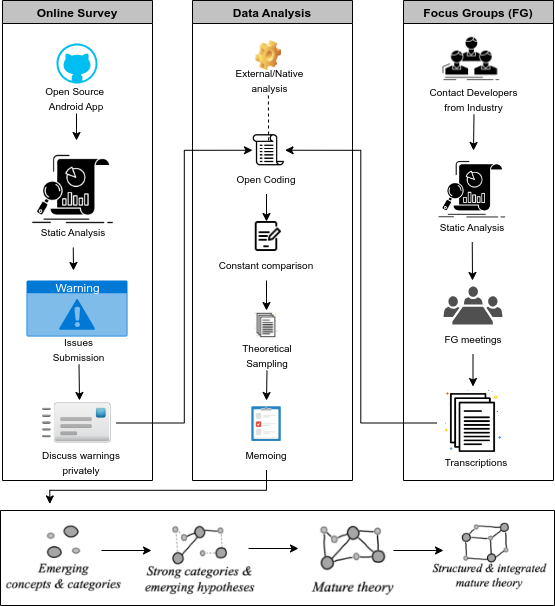
\includegraphics[scale=0.5]{img/metodologia.png}
  \caption{Metodologia adotada no artigo 'Perceptions of Software Practitioners Regarding Crypto-API Misuses and Vulnerabilities'}
  \label{averageWarnings}
\end{figure}


A imagem acima descreve a metodologia utilizada no artigo 'Perceptions of Software Practitioners Regarding Crypto-API Misuses and Vulnerabilities'. A metodologia abordada neste trabalho entra na etapa de 'Análise de Dados' em específico 'Análise externa / nativa', onde é feita a integração dos resultados obtidos pelo LibScout com os contextos fornecidos pelo CryptoGuard e CogniCrypt. Essa integração tenta proporcionar uma visão mais minuciosa e contextualizada de onde as vulnerabilidades identificadas se encontram.
Nosso trabalho propõe a seguinte integração:

\begin{figure}[!h]
  \centering
  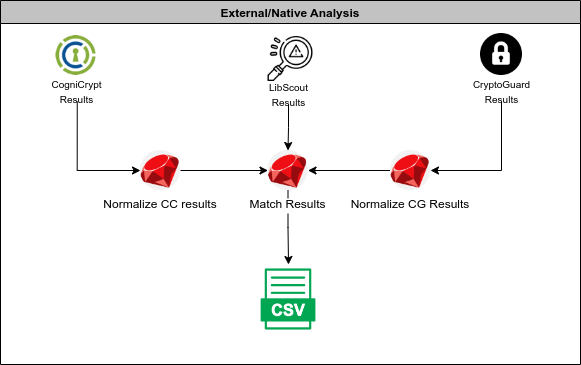
\includegraphics[scale=0.5]{img/studySettingsExternal.png}
  \caption{Metodologia adotada neste trabalho'}
  \label{averageWarnings}
\end{figure}

\begin{itemize}
\item{Coleta de Dados}
A metodologia adotada para a constituição do conjunto de dados envolveu uma cuidadosa seleção de aplicativos Java provenientes do renomado repositório F-Droid. Este último se destaca como um catálogo de aplicativos de código aberto e livre (FOSS), especialmente concebidos para a plataforma Android.

Nesse processo, buscou-se uma representativa diversidade de categorias de aplicativos, abrangendo áreas vitais como conectividade, finanças, segurança, mensagens de texto (SMS) e funcionalidades de sistema. Tal abordagem foi implementada com o intuito de assegurar uma abrangência abarcadora de contextos e finalidades, enriquecendo assim a robustez e representatividade do conjunto de dados analisado.

\item{Análise Estática}

A etapa subsequente consistiu na aplicação das ferramentas CryptoGuard e CogniCrypt para conduzir uma análise estática detalhada do código fonte dos aplicativos selecionados. Essa abordagem permitiu a identificação minuciosa de possíveis vulnerabilidades relacionadas às APIs criptográficas empregadas nos aplicativos avaliados. O uso dessas ferramentas especializadas proporcionou uma avaliação precisa e abrangente das práticas de segurança adotadas, visando aprimorar a integridade e robustez dos aplicativos em questão.

\item{Identificar a percepção de vulnerabilidade dos desenvoledores}

Após a conclusão da análise estática, foi possível identificar um conjunto de vulnerabilidades que não foram reconhecidas pelos desenvolvedores, bem como aquelas que foram identificadas, porém não receberam intervenção corretiva. Para facilitar a comunicação e o entendimento das questões de segurança identificadas, procedeu-se à criação de GISTS individuais para cada vulnerabilidade. Um GIST é um recurso que permite compartilhar trechos de código, arquivos inteiros ou até mesmo aplicações, e também possibilita a preservação e compartilhamento de saída de console ao executar, depurar ou testar o código. Cada GIST representa um repositório que pode ser clonado ou bifurcado por outras pessoas, promovendo assim a colaboração e a discussão ativa em busca do aprimoramento da segurança nos aplicativos avaliados.

\begin{figure}[!h]
  \centering
  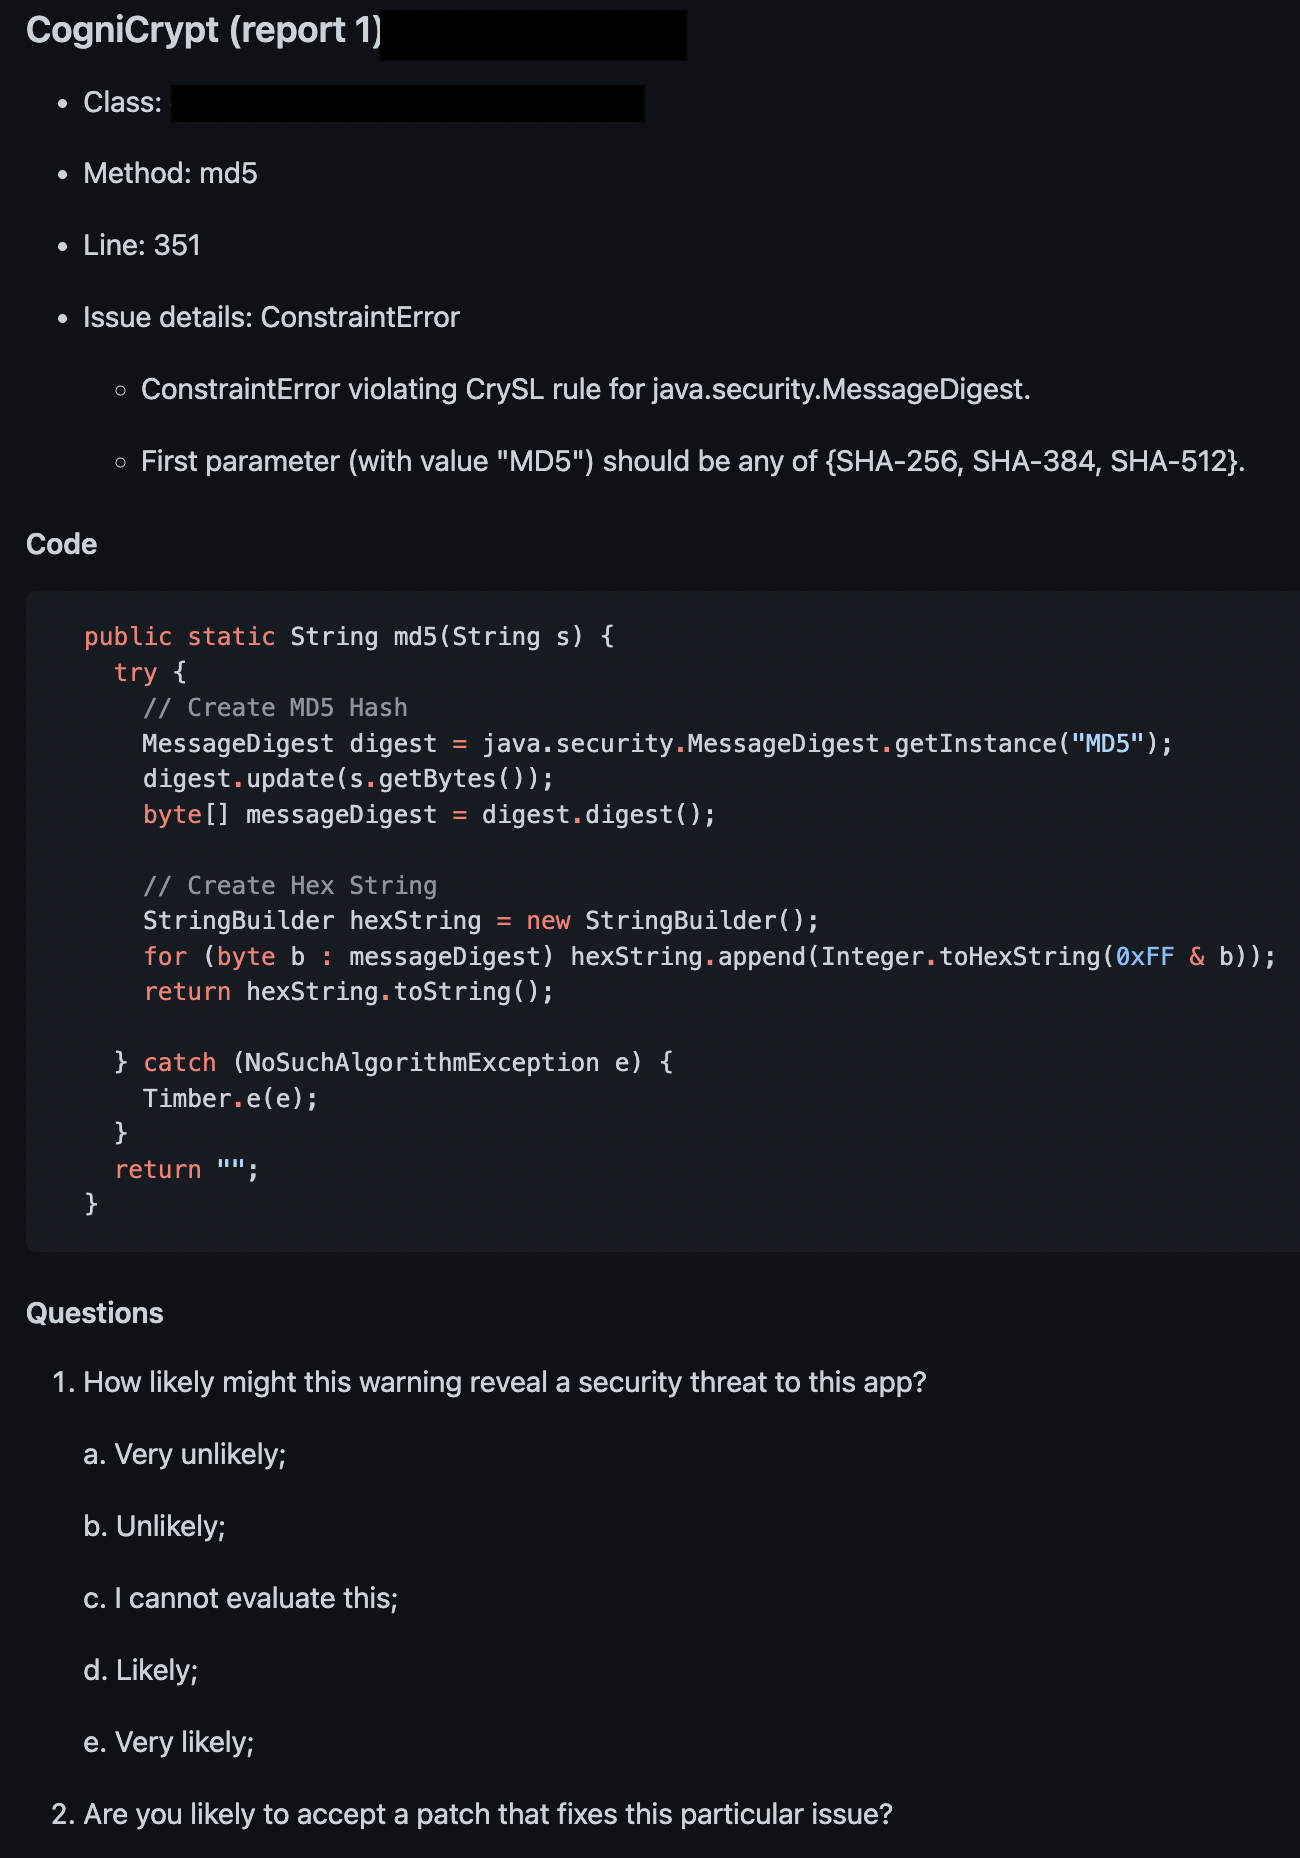
\includegraphics[scale=0.5]{img/gist.png}
  \caption{'Exemplo de uma Gist'}
  \label{averageWarnings}
\end{figure}

\item{Analisar origem das vulnerabilidades}

A etapa seguinte consistiu na análise da origem das vulnerabilidades identificadas. Para realizar essa análise, empregou-se a ferramenta LibScout, a qual desempenhou um papel crucial ao extrair informações detalhadas sobre as APIs criptográficas utilizadas nos aplicativos, permitindo, assim, a identificação de bibliotecas externas empregadas. A utilização do LibScout proporcionou um panorama abrangente das dependências externas dos aplicativos, fornecendo uma visão clara das fontes potenciais de vulnerabilidades no código. Esta abordagem foi essencial para direcionar os esforços na mitigação das ameaças identificadas e fortalecer a segurança das aplicações avaliadas.

A princípio, considerou-se a utilização do LibRadar devido à sua reputação pela rapidez de execução. Contudo, logo se constatou que a ferramenta estava baseada em dados disponibilizados até 2016, o que não condizia com nossa necessidade de informações atualizadas e abrangentes sobre as bibliotecas utilizadas nos aplicativos. Diante dessa constatação, optou-se por descartar o uso do LibRadar e buscar uma alternativa mais alinhada com os objetivos do estudo.

\item{Integração de Resultados}

Foi empreendido um esforço no sentido de desenvolver um processo de integração que possibilitasse a unificação dos resultados obtidos por meio do LibScout com os contextos fornecidos pelo CryptoGuard e CogniCrypt. Essa iniciativa tenta criar uma visão mais abrangente e contextualizada das vulnerabilidades identificadas. Em paralelo, foi realizada uma avaliação da eficácia dessa abordagem, no que tange à habilidade de determinar a origem dos alertas gerados pelas mencionadas ferramentas.

\end{itemize}

% Este capítulo oferece sugestões para produção de um documento descrevendo um Trabalho de Conclusão de curso...

% \section{UnB}%
% A \acrlong{UnB} oferece diversas informações em seu sítio\footnote{\url{http://www.unb.br/oportunidades/projeto_final_de_curso}}. O texto existente em 21/11/2014 é
% reproduzido a seguir:

% \fontshape{it}\selectfont%
% Os cursos de graduação, especialização e pós-graduação têm como objetivo formar o aluno e prepará-lo para o exercício profissional. Como avaliação do aprendizado, a universidade exige um projeto que mobiliza os estudantes a colaborar com a pesquisa acadêmica. Desde a escolha do tema até a apresentação do trabalho final, o tempo do aluno é ocupado quase integralmente. Para facilitar a vida desses estudantes, o Portal UnB preparou uma série de dicas de professores especialistas no assunto.

% \subsection{Os tipos}
% A monografia, a dissertação e a tese são, respectivamente, os trabalhos de conclusão de curso de graduação ou especialização, mestrado e doutorado. A grande diferença é a profundidade exigida no projeto, aumentada de acordo com a importância do título de cada nível acadêmico. Mas, em todos os casos, a pesquisa deve abordar o tema selecionado com coerência, consistência e referencial teórico adequado.

% Alguns cursos de graduação não exigem monografia, mas um relatório de estágios realizados, como acontece nas licenciaturas. A metodologia de pesquisar e apresentar resultados se mantém, como é exigido em todo projeto final.

% Uma monografia é, genericamente, um relatório de pesquisa sobre o assunto estudado. É específico a um tema pré-definido dentro de uma área de conhecimento e aborda questões e análises de um problema, a construção de uma teoria ou o desenvolvimento de um produto.

% Exigida no mestrado, a dissertação cobra do futuro mestre um conhecimento mais profundo. A pesquisa deve ser o resultado em relatório que representa o trabalho experimental ou exposição científica com um tema bem delimitado, e demonstrar o conhecimento de literatura existente sobre o assunto.

% A mais densa entre todos os projetos finais, a tese de doutorado exige mais no que diz respeito a teoria e metodologia do tema pesquisado. Deve apresentar contribuições reais para o desenvolvimento específico da especialidade em questão. A base do estudo demanda uma investigação original.

% \subsection{Teoria e prática}
% Todo projeto de conclusão de curso exige um relatório escrito baseado em teorias, mesmo que o assunto estudado seja algo prático como uma campanha publicitária ou um projeto arquitetônico. Porém, o inverso não se aplica.

% As divisões dos tipos de trabalho variam entre cada área de conhecimento. Em suma, o projeto pode ser teórico, prático ou uma união dos dois. Na primeira situação, o aluno pode fazer estudo de caso - pesquisar sobre um fato histórico ou evento importante - ou formular uma teoria - por meio de pesquisa ou reavaliação das semelhantes.

% O projeto prático se dedica a criação e construção de um produto, que pode variar de um novo motor a uma composição musical. O curso de graduação costuma oferecer a opção de um trabalho prático aos alunos. No caso dos cursos de mestrado e doutorado, nem todos os departamentos da universidade dispõem de linhas de pesquisa que permitam um projeto que vá além da teoria acadêmica.

% A união dos dois gêneros é comum quando o universitário relata a experiência de estágio ou na simulação de um projeto, como a construção de maquetes ou esquemas computacionais. As opções são vastas e o aluno deve explicar como e o que se deve fazer para que o projeto se torne possível.

% \subsection{Começo do projeto}
% Parece óbvio, mas muitos alunos esquecem a questão principal na hora de escolher o tema: o assunto deve interessar e estimular a pesquisa. Conviver meses com um tema que não agrada torna o trabalho mais complicado. Porém, escolher um bom tema não é abraçar e desenvolver sobre tudo que ele é e engloba. É preciso delimitar o assunto de forma específica.

% Um trabalho sobre a história do mundo, por exemplo, está fadado a se tornar superficial. Além de extremamente amplo, é grande o volume de informações a ser levantado e estudado. É importante ter foco para desenvolver um projeto coeso e com credibilidade.

% Além disso, o estudante necessita desenvolver um problema e traçar uma hipótese. Em um exemplo bem simples: a Guerra no Iraque (tema) e o terrorismo mundial (problema) – o aumento dos ataques depois da invasão americana (hipótese); ou seja, o que o aluno quer tratar e onde ele espera chegar na pesquisa. A não comprovação da hipótese não inviabiliza o trabalho, desde que o desenvolvimento da análise enriqueça os conhecimentos sobre o tema tratado.

% A prática essencial para o desenvolvimento de qualquer projeto é a pesquisa bibliográfica. As consultas às bibliotecas respaldam a parte teórica do estudo e podem elucidar diversas questões, sejam específicas do projeto ou sobre metodologias científicas. Nesse ponto, o papel do professor orientador é fundamental para a condução da pesquisa. Além da seleção dos livros, o docente analisa as melhores possibilidades de desenvolver o assunto, em todas as suas fases. Ele também pode indicar a aplicação de entrevistas e outros elementos de apoio ao conteúdo do projeto.

% Atualmente, o meio mais difundido de pesquisa é a Internet. Além de facilitar o acesso a documentos, pela rede é possível saber quanto o tema escolhido já foi objeto de estudo de outros acadêmicos. Mas essa facilidade deve ser utilizada para indicar um caminho.

% \subsection{Estrutura e regras}
% Antes do próprio trabalho escrito, o estudante deve fazer um projeto ou plano de pesquisa. O documento identifica o que deve ser feito, o porquê, como e onde será realizado o levantamento. Não há um modelo rígido para a apresentação do projeto de pesquisa, mas os seguintes elementos devem ser respondidos no texto:

% \begin{enumerate}
%   \item Definição do objeto de estudo (tema/problema da pesquisa)
%   \item Justificativa
%   \item Hipóteses de trabalho
%   \item Discussão teórica
%   \item Metodologia
%   \item Pesquisa Bibliográfica
% \end{enumerate}

% Seja monografia, dissertação ou tese, a parte escrita possui uma estrutura semelhante, embora cada uma tenha características próprias referentes à profundidade do tema estudado.

% De acordo com a Associação Brasileira de Normas Técnicas (ABNT), um trabalho acadêmico deve englobar os elementos pré-textuais (como resumo e índice), pós-textuais (bibliografia, anexos, entre outros) e textuais. Esses últimos compõem a parte central do trabalho - introdução, desenvolvimento e conclusão.

% A introdução é a parte inicial do texto e deve constar o objeto de pesquisa, os objetivos, a justificativa da escolha do tema e outras informações que sejam necessárias para esclarecer o assunto.

% A parte principal do trabalho está concentrada no desenvolvimento. É uma exposição sistematizada e ordenada de toda o estudo desenvolvido, apresentando análise e interpretação das informações e dados obtidos. A conclusão é a etapa final do texto. Nela, são apresentados os resultados tendo como referência os objetivos e hipóteses da pesquisa.

% Em todo o trabalho a linguagem utilizada deve ser interessante, sem apelar para a linguagem coloquial. O trabalho deve estar de acordo com as normas da ABNT. Procure livros sobre estrutura e regras do tipo de projeto final específico de seu interesse.

% \subsection{O projeto está pronto. E agora?}
% Após a finalização do projeto, chega o momento de preparar a apresentação. Em geral, a banca examinadora é formada por três docentes, sendo um deles o professor orientador do projeto. Também é comum aos alunos o direito de escolha dos avaliadores, desde que seja pertinente ao assunto e ao objetivo do estudo.

% Esses professores recomendam uma apresentação resumida do projeto, pontuando as características essenciais e como se chegou às conclusões. É sempre bom explicar o cronograma de todo o trabalho. É preciso, também, ficar atento ao tempo. Não é necessário explicar os conceitos já citados no projeto e pode influenciar a nota final. Lembre-se que as explicações são voltadas para os avaliadores, que já leram o seu trabalho.

% Durante as considerações da banca examinadora não se deve interromper a avaliação dos professores, exceto quando eles dirigirem diretamente uma pergunta ao aluno. Educação e conhecimento dos procedimentos acadêmicos são essenciais para uma boa apresentação. Após a avaliação, os professores pedem para os presentes se retirarem da sala. É feita uma reunião onde será decidida a nota do projeto.

% Cada departamento possui regras e orientações para a apresentação dos trabalhos de conclusão. Cabe ao aluno perguntar à coordenação do curso e ao orientador todas as etapas do processo de elaboração do projeto final.

% \fontshape{n}\selectfont%
